\chapter{Quantifying MGXS Approximations}
\label{chap:biases}

%%%%%%%%%%%%%%%%%%%%%%%%%%%%%%%%%%%%%%%%%%%%%%%%%%%%%%%%%%%%%%%%%%%%%%%%%%%%%%%%
\section{Introduction}
\label{sec:chap4-intro}

\begin{itemize}[noitemsep]
  \item quantify \ac{MGXS} different approximation errors
  \item leave intra-pin spatial self-shielding error for later section
  \item need to discuss difference between iso-in-lab and regular scattering
\end{itemize}


%%%%%%%%%%%%%%%%%%%%%%%%%%%%%%%%%%%%%%%%%%%%%%%%%%%%%%%%%%%%%%%%%%%%%%%%%%%%%%%%
\section{Case Studies}
\label{sec:chap4-case-studies}

\begin{itemize}[noitemsep]
  \item \ac{MOC} convergence studies with \ac{MC}-generated \ac{MGXS}
  \begin{itemize}[noitemsep]
    \item track discretization - \# azimuthal angles,  track spacing
    \item \# energy groups
    \item spatial discretization
  \end{itemize}
  \item compare to reference \ac{MC} solution:
  \begin{itemize}
    \item eigenvalue
	\item Define $\Delta\rho$
    \item fluxes
  \end{itemize}
\end{itemize}

\begin{equation}
\label{eqn:chap4-delta-rho}
\Delta\rho = \left(k_{eff}^{OpenMOC} - k_{eff}^{OpenMC}\right) \times 1E5
\end{equation}

%%%%%%%%%%%%%%%%%%%%%%%%%%%%
\subsection{Infinite Medium}
\label{subsec:chap4-inf-medium}

\begin{itemize}[noitemsep]
\item 128 azim angles
\item 0.01 cm track spacing
\item 1E-7 convergence threshold
\item double precision
\end{itemize}

\begin{table}[h!]
  \centering
  \caption{Infinite medium isotopic composition.}
  \label{table:chap2-inf-med-isotopes} 
  \vspace{14pt}
  \begin{tabular}{c c}
  \toprule
  \multicolumn{1}{c}{\bf Nuclide} &
  \multicolumn{1}{c}{\bf Density [g/cc]} \\
  \midrule
  H-1 & 2.8999E-2 \\
  O-16 & 1.4501E-2 \\
  Zr-90 & 2.1160E-3 \\  
  U-235 & 1.1414E-4 \\
  U-238 & 6.8860E-3 \\
  \bottomrule
\end{tabular}
\end{table}

\begin{table}[h!]
  \centering
  \caption{Reference $k_{eff}$ for an infinite medium.}
  \label{table:chap2-inf-med-reference} 
  \vspace{14pt}
  \begin{tabular}{c c}
  \toprule
  \multicolumn{1}{c}{\bf Anisotropic} &
  \multicolumn{1}{c}{\bf Isotropic in Lab} \\
  \midrule
  1.15908 $\pm$ 0.00001 & 1.15907 $\pm$ 0.00001 \\
  \bottomrule
\end{tabular}
\end{table}

\begin{table}[h!]
  \centering
  \caption{Angular-dependent $k_{eff}$ bias for an infinite medium.}
  \label{table:chap2-inf-med-angle}
  \vspace{14pt}
  \begin{tabular}{c S[table-format=2.1] S[table-format=2.1] S[table-format=2.1] c S[table-format=2.1] S[table-format=2.1] S[table-format=2.1]} 
  \toprule
  & \multicolumn{7}{c}{\boldmath $\Delta\rho$ {\bf [pcm]}} \\
  \midrule
  \multicolumn{1}{c}{\bf \# Angles} &
  \multicolumn{1}{c}{\bf 0.1 cm} & 
  \multicolumn{1}{c}{\bf 0.01 cm} & 
  \multicolumn{1}{c}{\bf 0.001 cm} &
  \multicolumn{1}{c}{} &
  \multicolumn{1}{c}{\bf 0.1 cm} & 
  \multicolumn{1}{c}{\bf 0.01 cm} & 
  \multicolumn{1}{c}{\bf 0.001 cm} \\
  \midrule
  & \multicolumn{3}{c}{\bf No Transport Corr.} &
  \multicolumn{1}{c}{} &
  \multicolumn{3}{c}{\bf Isotropic in Lab} \\
  \cline{2-4} \cline{6-8}
4 & 1.3 & 1.3 & 1.3 & & -0.1 & -0.1 & -0.1 \\
8 & 1.3 & 1.3 & 1.3 & & -0.1 & -0.1 & -0.1 \\
16 & 1.3 & 1.3 & 1.3 & & -0.1 & -0.1 & -0.1 \\
32 & 1.3 & 1.3 & 1.3 & & -0.1 & -0.1 & -0.1 \\
64 & 1.3 & 1.3 & 1.3 & & -0.1 & -0.1 & -0.1 \\
128 & 1.3 & 1.3 & 1.3 & & -0.1 & -0.1 & -0.1 \\
  \bottomrule
\end{tabular}
\end{table}

\begin{table}[h!]
  \centering
  \caption{Energy-dependent $k_{eff}$ bias for an infinite medium.}
  \label{table:chap2-inf-med-energy} 
  \vspace{14pt}
  \begin{tabular}{c S[table-format=2.1] S[table-format=2.1]}
  \toprule
  \multicolumn{1}{c}{\textbf{\# Groups}} &
  \multicolumn{2}{c}{\boldmath $\Delta\rho$ {\bf [pcm]}} \\
  \midrule
  & \multicolumn{1}{c}{\bf No Transport Corr.} &
  \multicolumn{1}{c}{\bf Isotropic in Lab} \\
  \midrule
1 & -11.1 & -10.5 \\
2 & -9.5 & -7.1 \\
4 & -0.1 & -0.5 \\
8 & 0.3 & -0.0 \\
16 & -0.2 & 0.5 \\
25 & 1.8 & 0.1 \\
40 & 1.6 & 0.1 \\
70 & 1.3 & -0.1 \\
  \bottomrule
\end{tabular}
\end{table}


%%%%%%%%%%%%%%%%%%%%
\subsection{1D Slab}
\label{subsec:chap4-slab}

\begin{table}[h!]
  \centering
  \caption{1D slab isotopic composition.}
  \label{table:chap2-slab-isotopes} 
  \vspace{14pt}
  \begin{tabular}{c c}
  \toprule
  \multicolumn{1}{c}{\bf Nuclide} &
  \multicolumn{1}{c}{\bf Density [g/cc]} \\
  \midrule
  \multicolumn{2}{c}{\bf UO$_2$ Fuel} \\
  \midrule
  O-16 & 4.5764E-2 \\
  U-235 & 7.1813E-4 \\
  U-238 & 2.2154E-2 \\
  \midrule
  \multicolumn{2}{c}{\bf Zircaloy Cladding} \\
  \midrule
  Zr-90 & 2.1886E-2 \\
  Zr-91 & 4.7729E-3 \\
  Zr-92 & 7.2955E-3 \\
  Zr-94 & 7.3933E-3 \\
  Zr-96 & 1.1911E-3 \\
  \midrule
  \multicolumn{2}{c}{\bf Borated Water}  \\
  \midrule
  H-1 & 4.4145E-2 \\
  B-10 & 9.5253E-6 \\
  B-11 & 3.8340E-5 \\
  O-16 & 2.2072E-2 \\
  \bottomrule
\end{tabular}
\end{table}

\begin{figure}[h!]
\begin{subfigure}{\textwidth}
  \centering
  
\includegraphics[width=\linewidth]{figures/biases/slab/slab-simple}
  \caption{}
\end{subfigure} \\
\begin{subfigure}{\textwidth}
  \centering
  
\includegraphics[width=\linewidth]{figures/biases/slab/slab-8x}
  \caption{}
\end{subfigure}
\caption[1D slab materials and geometry]{A 1D slab with fuel, clad and moderator (a). Linearly-spaced tally zones were defined in each material in OpenMC and as flat source regions in OpenMOC (b).}
\label{fig:chap4-slab}
\end{figure}

\begin{itemize}[noitemsep]
  \item 1D slab equivalent to a representative \ac{PWR} fuel pin
  \item 128 azim angles
  \item 0.01 cm track spacing
  \item 1E-7 convergence threshold
  \item double precision
\end{itemize}

\begin{table}[h!]
  \centering
  \caption{Reference $k_{eff}$ for an 1D slab.}
  \label{table:chap2-slab-reference} 
  \vspace{14pt}
  \begin{tabular}{c c}
  \toprule
  \multicolumn{1}{c}{\bf Anisotropic} &
  \multicolumn{1}{c}{\bf Isotropic in Lab} \\
  \midrule
  1.01073 $\pm$ 0.00003 & 0.96284 $\pm$ 0.00003 \\
  \bottomrule
\end{tabular}
\end{table}

\begin{table}[h!]
  \centering
  \caption{Angular-dependent $k_{eff}$ bias for a 1D slab.}
  \label{table:chap2-slab-angle}
  \vspace{14pt}
  \begin{tabular}{c S[table-format=6.1] S[table-format=6.1] S[table-format=6.1] c S[table-format=6.1] S[table-format=6.1] S[table-format=6.1]} 
  \toprule
  & \multicolumn{7}{c}{\boldmath $\Delta\rho$ {\bf [pcm]}} \\
  \midrule
  \multicolumn{1}{c}{\bf \# Angles} &
  \multicolumn{1}{c}{\bf 0.1 cm} & 
  \multicolumn{1}{c}{\bf 0.01 cm} & 
  \multicolumn{1}{c}{\bf 0.001 cm} &
  \multicolumn{1}{c}{} &
  \multicolumn{1}{c}{\bf 0.1 cm} & 
  \multicolumn{1}{c}{\bf 0.01 cm} & 
  \multicolumn{1}{c}{\bf 0.001 cm} \\
  \midrule
  & \multicolumn{3}{c}{\bf No Transport Corr.} &
  \multicolumn{1}{c}{} &
  \multicolumn{3}{c}{\bf Isotropic in Lab} \\
  \cline{2-4} \cline{6-8}
4 & 12040 & 12177 & 12177 & & 16843 & 16980 & 16980 \\
8 & 10660 & 10666 & 10664 & & 15462 & 15468 & 15466 \\
16 & 10433 & 10433 & 10431 & & 15235 & 15235 & 15233 \\
32 & 10386 & 10385 & 10384 & & 15188 & 15186 & 15185 \\
64 & 10377 & 10377 & 10377 & & 15178 & 15179 & 15179 \\
128 & 10376 & 10375 & 10375 & & 15178 & 15177 & 15177 \\
  \bottomrule
\end{tabular}
\end{table}

\begin{table}[h!]
  \centering
  \caption{Energy-dependent $k_{eff}$ bias for a 1D slab.}
  \label{table:chap2-slab-energy} 
  \vspace{14pt}
  \begin{tabular}{c S[table-format=6.1] S[table-format=6.1] S[table-format=6.1] S[table-format=6.1] S[table-format=6.1]}
  \toprule
  & \multicolumn{5}{c}{\boldmath $\Delta\rho$ {\bf [pcm]}} \\
  \midrule  
  \multicolumn{1}{c}{\textbf{\# Groups}} &
  \multicolumn{1}{c}{\bf 1$\times$} &
  \multicolumn{1}{c}{\bf 2$\times$} &
  \multicolumn{1}{c}{\bf 4$\times$} &
%  \multicolumn{1}{c}{\bf 8$\times$} &
  \multicolumn{1}{c}{\bf 16$\times$} &
  \multicolumn{1}{c}{\bf 32$\times$} \\
  \midrule
  & \multicolumn{5}{c}{\bf No Transport Corr.} \\
  \cline{2-6}
1 & 4241 & 4640 & 4932 & 5084 & 5094 \\
2 & 8786 & 4998 & 734 & -2486 & -2732 \\
4 & 8972 & 4685 & -222 & -3925 & -4207 \\
8 & 10069 & 5382 & -73 & -4337 & -4671 \\
16 & 10172 & 5479 & 43 & -4219 & -4555 \\
25 & 10250 & 5525 & -36 & -4410 & -4755 \\
40 & 10355 & 5609 & 17 & -4395 & -4745 \\
70 & 10375 & 5636 & 31 & -4398 & -4750 \\
  & \multicolumn{5}{c}{\bf With Transport Corr.} \\
  \cline{2-6}
1 & 4041 & 4263 & 4383 & 4435 & 4438 \\
2 & 9201 & 5755 & 2525 & 497 & 358 \\
4 & 9134 & 5365 & 1868 & -312 & -462 \\
8 & 10296 & 6284 & 2347 & -305 & -497 \\
16 & 10417 & 6441 & 2566 & -75 & -269 \\
25 & 10376 & 6385 & 2480 & -181 & -381 \\
40 & 10474 & 6471 & 2550 & -140 & -344 \\
70 & 10482 & 6486 & 2569 & -124 & -329 \\
  & \multicolumn{5}{c}{\bf Isotropic in Lab} \\
  \cline{2-6}
1 & 4654 & 5126 & 5480 & 5668 & 5680 \\
2 & 13926 & 10000 & 5563 & 2201 & 1943 \\
4 & 13752 & 9389 & 4388 & 604 & 315 \\
8 & 15103 & 10367 & 4861 & 560 & 223 \\
16 & 15194 & 10452 & 4968 & 672 & 332 \\
25 & 15089 & 10350 & 4774 & 389 & 42 \\
40 & 15165 & 10413 & 4813 & 396 & 46 \\
70 & 15177 & 10435 & 4827 & 396 & 44 \\
  \bottomrule
\end{tabular}
\end{table}

\begin{table}[h!]
  \centering
  \caption{Spatial-dependent $k_{eff}$ bias for a 1D slab.}
  \label{table:chap2-slab-space} 
  \vspace{14pt}
  \begin{tabular}{c S[table-format=6.1] S[table-format=6.1] S[table-format=6.1] S[table-format=6.1] S[table-format=6.1]}
  \toprule
  & \multicolumn{5}{c}{\boldmath $\Delta\rho$ {\bf [pcm]}} \\
  \midrule  
  \multicolumn{1}{c}{\textbf{\# Groups}} &
  \multicolumn{1}{c}{\bf 1$\times$} &
  \multicolumn{1}{c}{\bf 2$\times$} &
  \multicolumn{1}{c}{\bf 4$\times$} &
%  \multicolumn{1}{c}{\bf 8$\times$} &
  \multicolumn{1}{c}{\bf 16$\times$} &
  \multicolumn{1}{c}{\bf 32$\times$} \\
  \midrule
  & \multicolumn{5}{c}{\bf No Transport Corr.} \\
  \cline{2-6}
1 & 4253 & 4750 & 5094 & 5263 & 5271 \\
2 & 8797 & 4796 & 404 & -2817 & -3062 \\
4 & 8983 & 4754 & -65 & -3610 & -3876 \\
8 & 10080 & 5329 & -201 & -4491 & -4826 \\
16 & 10184 & 5422 & -92 & -4401 & -4742 \\
25 & 10262 & 5519 & -63 & -4436 & -4780 \\
40 & 10366 & 5611 & 4 & -4411 & -4758 \\
70 & 10387 & 5633 & 19 & -4406 & -4756 \\
  & \multicolumn{5}{c}{\bf With Transport Corr.} \\
  \cline{2-6}
1 & 4052 & 4338 & 4475 & 4541 & 4544 \\
2 & 9212 & 5615 & 2393 & 470 & 346 \\
4 & 9145 & 5475 & 2172 & 201 & 72 \\
8 & 10308 & 6245 & 2277 & -363 & -550 \\
16 & 10429 & 6405 & 2490 & -164 & -356 \\
25 & 10387 & 6380 & 2464 & -193 & -388 \\
40 & 10486 & 6472 & 2543 & -147 & -348 \\
70 & 10494 & 6483 & 2561 & -130 & -332 \\
  & \multicolumn{5}{c}{\bf Isotropic in Lab} \\
  \cline{2-6}
1 & 4654 & 5303 & 5731 & 5972 & 6011 \\
2 & 13926 & 9470 & 4647 & 1130 & 883 \\
4 & 13752 & 9266 & 4241 & 540 & 266 \\
8 & 15103 & 10190 & 4546 & 169 & -165 \\
16 & 15194 & 10282 & 4658 & 269 & -68 \\
25 & 15089 & 10319 & 4723 & 322 & -17 \\
40 & 15165 & 10395 & 4783 & 351 & 9 \\
70 & 15177 & 10416 & 4803 & 370 & 29 \\
  \bottomrule
\end{tabular}
\end{table}

-add figure for flux comparisons\\

%%%%%%%%%%%%%%%%%%%%%%%%%%%%%
\subsection{2D Fuel Pin Cell}
\label{subsec:chap4-pin}

\begin{table}[h!]
  \centering
  \caption{2D fuel pin isotopic composition.}
  \label{table:chap2-pin-isotopes} 
  \vspace{14pt}
  \begin{tabular}{c c}
  \toprule
  \multicolumn{1}{c}{\bf Nuclide} &
  \multicolumn{1}{c}{\bf Atom Density [ao]} \\
  \midrule
  \multicolumn{2}{c}{\bf UO$_2$ Fuel} \\
  \midrule
  O-16 & 4.5829E-2 \\
  U-235 & 5.5815E-4 \\
  U-238 & 2.2408E-2 \\
  \midrule
  \multicolumn{2}{c}{\bf Helium Gap} \\
  \midrule
  He-4 & 2.4044E-4 \\
  \midrule
  \multicolumn{2}{c}{\bf Zircaloy Cladding} \\
  \midrule
  O-16 & 3.0743E-4 \\
  Fe-56 & 1.3610E-4 \\
  Zr-90 & 2.1827E-2 \\
  \midrule
  \multicolumn{2}{c}{\bf Borated Water}  \\
  \midrule
  H-1 & 4.9457E-2 \\
  B-10 & 8.0042E-6 \\
  B-11 & 3.2218E-5 \\
  O-16 & 2.4672E-2 \\
  \bottomrule
\end{tabular}
\end{table}

\begin{table}[h!]
  \centering
  \caption{2D fuel pin material densities.}
  \label{table:chap2-pin-densities} 
  \vspace{14pt}
  \begin{tabular}{c c}
  \toprule
  \multicolumn{1}{c}{\bf Material} &
  \multicolumn{1}{c}{\bf Density [g/cc]} \\
  \midrule
  UO$_2$ Fuel & 1.03E+1 \\
  Hellium & 1.59E-3 \\
  Zircaloy & 6.55E+0 \\
  Borated Water & 7.41E-1 \\   
  \bottomrule
\end{tabular}
\end{table}

\begin{figure}[h!]
\begin{subfigure}{.33\textwidth}
  \centering
  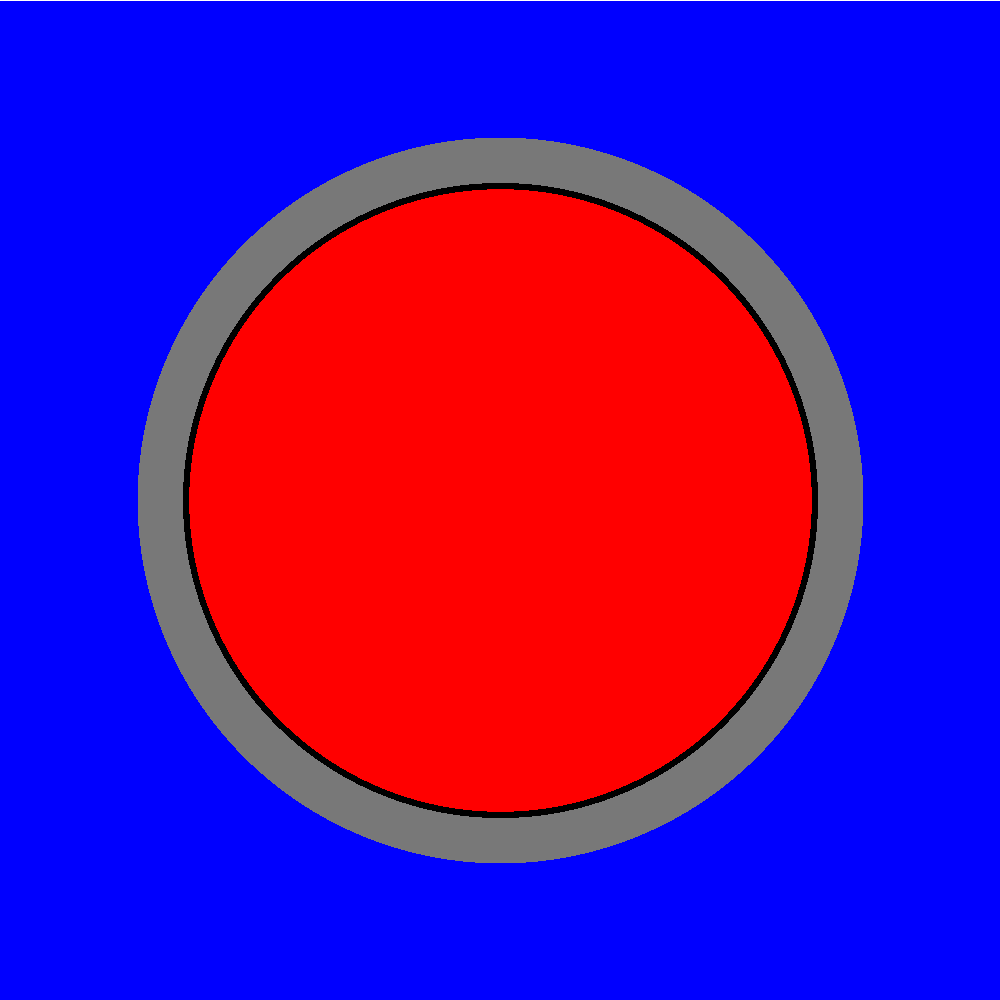
\includegraphics[width=0.9\linewidth]{figures/biases/pin-cell/pin-cell-simple}
  \caption{}
\end{subfigure}%
\begin{subfigure}{.33\textwidth}
  \centering
  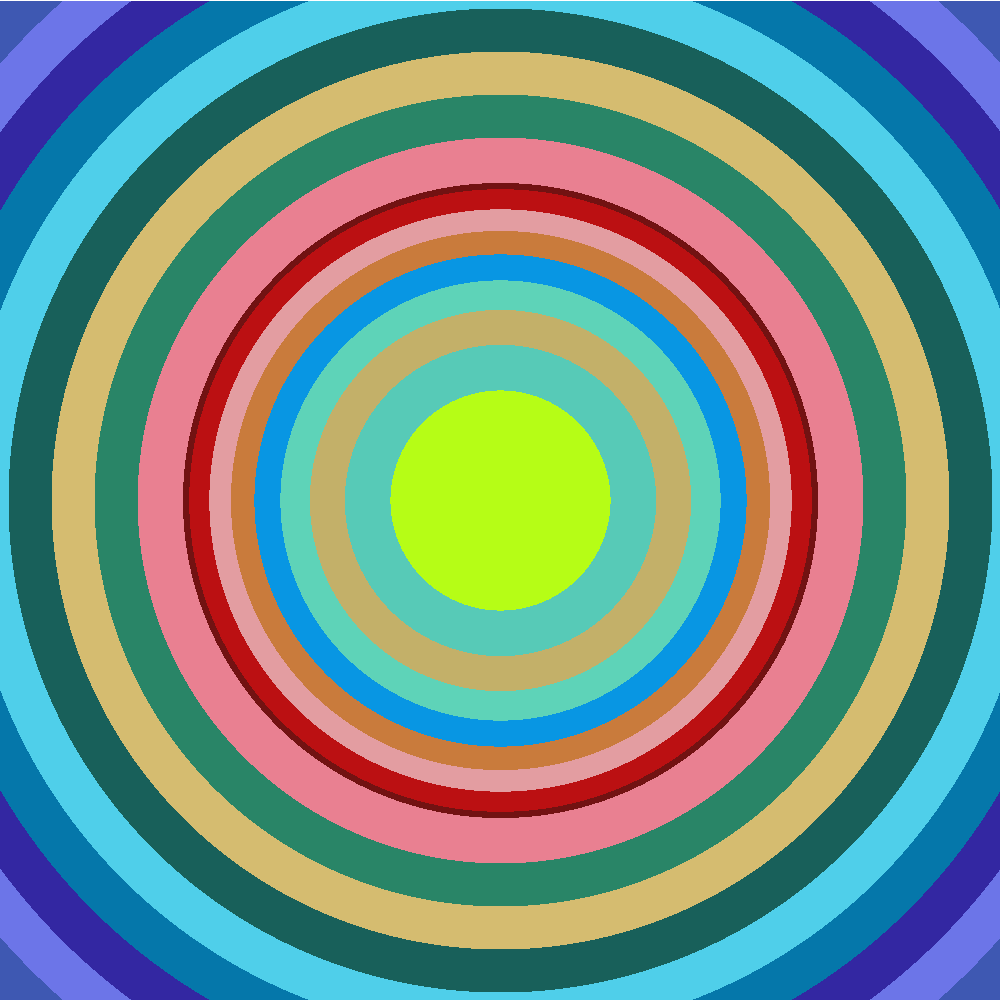
\includegraphics[width=0.9\linewidth]{figures/biases/pin-cell/pin-cell-8x}
  \caption{}
\end{subfigure}
\begin{subfigure}{.33\textwidth}
  \centering
  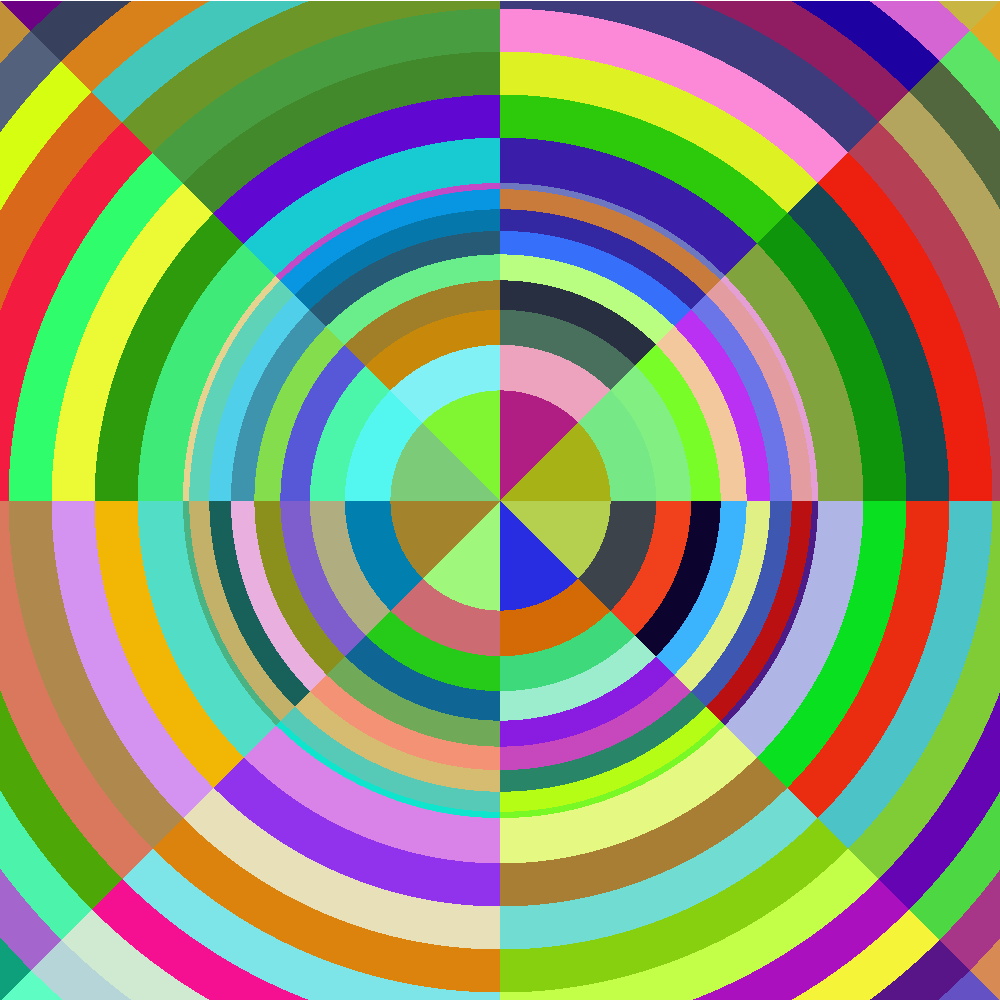
\includegraphics[width=0.9\linewidth]{figures/biases/pin-cell/pin-cell-8x8}
  \caption{}
\end{subfigure}
\caption[Pin cell materials and geometry]{A PWR fuel pin cell with fuel, gap, clad and moderator (a). Radial tally zones were defined in each material in OpenMC (b). The tally zones were further subdivided into angular sectors for the flat source region mesh in OpenMOC (c).}
\label{fig:chap4-pin-cell}
\end{figure}

\begin{table}[h!]
  \centering
  \caption{Reference $k_{eff}$ for an 2D fuel pin.}
  \label{table:chap2-pin-reference} 
  \vspace{14pt}
  \begin{tabular}{c c}
  \toprule
  \multicolumn{1}{c}{\bf Anisotropic} &
  \multicolumn{1}{c}{\bf Isotropic in Lab} \\
  \midrule
  1.17486 $\pm$ 0.00003 & 1.17421 $\pm$ 0.00002 \\
  \bottomrule
\end{tabular}
\end{table}

\begin{table}[h!]
  \centering
  \caption{Angular-dependent $k_{eff}$ bias for a 2D fuel pin.}
  \label{table:chap2-pin-angle}
  \vspace{14pt}
  \begin{tabular}{c S[table-format=2.1] S[table-format=2.1] S[table-format=2.1] c S[table-format=2.1] S[table-format=2.1] S[table-format=2.1]} 
  \toprule
  & \multicolumn{7}{c}{\boldmath $\Delta\rho$ {\bf [pcm]}} \\
  \midrule
  \multicolumn{1}{c}{\bf \# Angles} &
  \multicolumn{1}{c}{\bf 0.1 cm} & 
  \multicolumn{1}{c}{\bf 0.01 cm} & 
  \multicolumn{1}{c}{\bf 0.001 cm} &
  \multicolumn{1}{c}{} &
  \multicolumn{1}{c}{\bf 0.1 cm} & 
  \multicolumn{1}{c}{\bf 0.01 cm} & 
  \multicolumn{1}{c}{\bf 0.001 cm} \\
  \midrule
  & \multicolumn{3}{c}{\bf No Transport Corr.} &
  \multicolumn{1}{c}{} &
  \multicolumn{3}{c}{\bf Isotropic in Lab} \\
  \cline{2-4} \cline{6-8}
4 & 365 & 390 & 391 & & 460 & 484 & 486 \\
8 & -251 & -289 & -285 & & -157 & -194 & -191 \\
16 & -297 & -263 & -266 & & -202 & -168 & -171 \\
32 & -180 & -196 & -188 & & -86 & -101 & -94 \\
64 & -112 & -154 & -143 & & -18 & -60 & -49 \\
128 & -139 & -134 & -125 & & -45 & -39 & -31 \\
256 & -131 & -125 & -123 & & -36 & -30 & -28 \\
512 & -124 & -121 & -122 & & -30 & -27 & -28 \\
  \bottomrule
\end{tabular}
\end{table}

\begin{table}[h!]
  \centering
  \caption{Energy-dependent $k_{eff}$ bias for a 2D fuel pin.}
  \label{table:chap2-pin-energy} 
  \vspace{14pt}
  \begin{tabular}{c S[table-format=6.1] S[table-format=6.1] S[table-format=6.1] S[table-format=6.1] S[table-format=6.1]}
  \toprule
  & \multicolumn{5}{c}{\boldmath $\Delta\rho$ {\bf [pcm]}} \\
  \midrule  
  \multicolumn{1}{c}{\textbf{\# Groups}} &
  \multicolumn{1}{c}{\bf 1$\times$} &
  \multicolumn{1}{c}{\bf 2$\times$} &
  \multicolumn{1}{c}{\bf 4$\times$} &
  \multicolumn{1}{c}{\bf 8$\times$} &
  \multicolumn{1}{c}{\bf 16$\times$} \\
  \midrule
  & \multicolumn{5}{c}{\bf No Transport Corr.} \\
  \cline{2-6}
1 & 77 & 78 & 78 & 78 & 78 \\
2 & 34 & -10 & -40 & -52 & -50 \\
4 & -55 & -95 & -123 & -137 & -145 \\
8 & -71 & -131 & -177 & -198 & -208 \\
16 & -68 & -135 & -188 & -212 & -223 \\
25 & -126 & -189 & -241 & -267 & -275 \\
40 & -129 & -197 & -253 & -282 & -290 \\
70 & -129 & -200 & -259 & -289 & -298 \\
  & \multicolumn{5}{c}{\bf Transport Corr.} \\
  \cline{2-6}
1 & 63 & 64 & 64 & 64 & 63 \\
2 & 52 & 22 & 4 & -2 & 6 \\
4 & -60 & -89 & -108 & -125 & -126 \\
8 & -75 & -123 & -157 & -180 & -183 \\
16 & -68 & -123 & -165 & -191 & -194 \\
25 & -128 & -182 & -225 & -250 & -253 \\
40 & -133 & -192 & -241 & -268 & -272 \\
70 & -135 & -196 & -248 & -277 & -281 \\
  & \multicolumn{5}{c}{\bf Isotropic in Lab} \\
  \cline{2-6}
1 & 91 & 92 & 92 & 93 & 92 \\
2 & 153 & 109 & 78 & 67 & 69 \\
4 & 31 & -9 & -38 & -51 & -59 \\
8 & 31 & -29 & -75 & -95 & -106 \\
16 & 41 & -26 & -79 & -103 & -114 \\
25 & -27 & -91 & -142 & -169 & -177 \\
40 & -34 & -103 & -159 & -187 & -196 \\
70 & -35 & -106 & -165 & -195 & -204 \\
  \bottomrule
\end{tabular}
\end{table}

\begin{table}[h!]
  \centering
  \caption{Spatial-dependent $k_{eff}$ bias for a 2D fuel pin.}
  \label{table:chap2-pin-space} 
  \vspace{14pt}
  \begin{tabular}{c S[table-format=6.1] S[table-format=6.1] S[table-format=6.1] S[table-format=6.1] S[table-format=6.1]}
  \toprule
  & \multicolumn{5}{c}{\boldmath $\Delta\rho$ {\bf [pcm]}} \\
  \midrule  
  \multicolumn{1}{c}{\textbf{\# Groups}} &
  \multicolumn{1}{c}{\bf 1$\times$} &
  \multicolumn{1}{c}{\bf 2$\times$} &
  \multicolumn{1}{c}{\bf 4$\times$} &
  \multicolumn{1}{c}{\bf 8$\times$} &
  \multicolumn{1}{c}{\bf 16$\times$} \\
  \midrule
  & \multicolumn{5}{c}{\bf No Transport Corr.} \\
  \cline{2-6}
 & 79 & 78 & 62 & 62 & 53 \\
2 & 36 & -7 & -57 & -93 & -92 \\
4 & -53 & -90 & -136 & -173 & -184 \\
8 & -70 & -127 & -190 & -240 & -247 \\
16 & -66 & -130 & -198 & -255 & -257 \\
25 & -124 & -189 & -257 & -321 & -324 \\
40 & -127 & -200 & -272 & -339 & -344 \\
70 & -128 & -204 & -278 & -347 & -353 \\
  & \multicolumn{5}{c}{\bf With Transport Corr.} \\
  \cline{2-6}
1 & 65 & 79 & 74 & 30 & 33 \\
2 & 54 & 34 & 4 & -45 & -33 \\
4 & -58 & -77 & -106 & -166 & -165 \\
8 & -73 & -111 & -159 & -227 & -227 \\
16 & -66 & -111 & -168 & -238 & -240 \\
25 & -126 & -178 & -238 & -310 & -310 \\
40 & -131 & -188 & -256 & -330 & -331 \\
70 & -133 & -193 & -263 & -339 & -340 \\
  & \multicolumn{5}{c}{\bf Isotropic in Lab} \\
  \cline{2-6}
1 & 92 & 109 & 54 & 48 & 28 \\
2 & 154 & 107 & 28 & 12 & -6 \\
4 & 32 & -3 & -52 & -91 & -107 \\
8 & 32 & -22 & -93 & -136 & -152 \\
16 & 42 & -23 & -99 & -147 & -161 \\
25 & -26 & -95 & -169 & -220 & -238 \\
40 & -33 & -104 & -186 & -241 & -259 \\
70 & -34 & -107 & -193 & -247 & -267 \\
  \bottomrule
\end{tabular}
\end{table}

-make plots without SPH\\

\begin{figure}[h!]
  \centering
  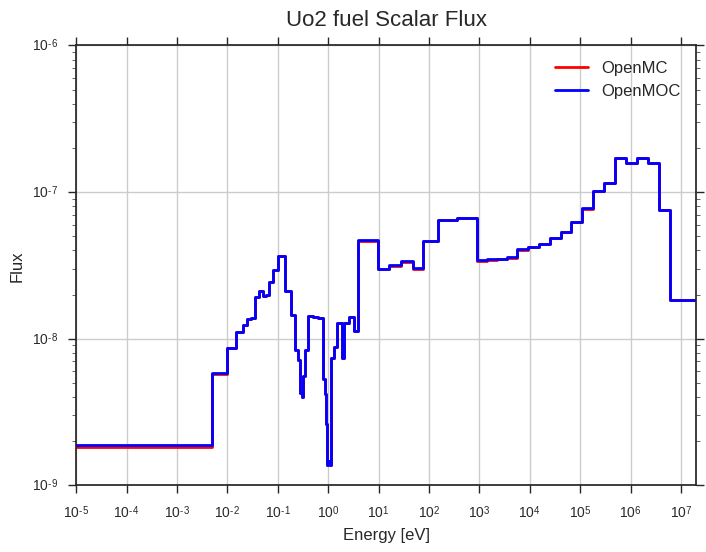
\includegraphics[width=0.9\linewidth]{figures/biases/pin-cell/flux-uo2-fuel}
  \caption{}
\label{fig:chap2-pin-flux}
\end{figure}

\begin{figure}[h!]
  \centering
  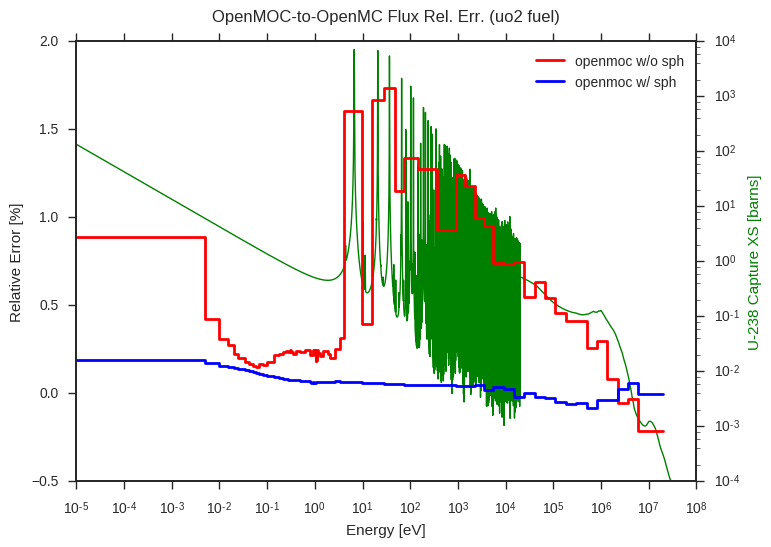
\includegraphics[width=0.9\linewidth]{figures/biases/pin-cell/rel-err-uo2-fuel}
  \caption{}
\label{fig:chap2-pin-flux}
\end{figure}


%%%%%%%%%%%%%%%%%%%%%%%%%%%%%%%%%%%%%%%%%%%
\subsection{2D Fuel Assembly}

\begin{table}[h!]
  \centering
  \caption{Reference $k_{eff}$ for an 2D fuel assembly.}
  \label{table:chap2-lattice-reference} 
  \vspace{14pt}
  \begin{tabular}{c c}
  \toprule
  \multicolumn{1}{c}{\bf Anisotropic} &
  \multicolumn{1}{c}{\bf Isotropic in Lab} \\
  \midrule
  \bottomrule
\end{tabular}
\end{table}

\begin{table}[h!]
  \centering
  \caption{Angular-dependent $k_{eff}$ bias for a 2D fuel assembly.}
  \label{table:chap2-lattice-angle}
  \vspace{14pt}
  \begin{tabular}{c S[table-format=2.1] S[table-format=2.1] S[table-format=2.1] c S[table-format=2.1] S[table-format=2.1] S[table-format=2.1]} 
  \toprule
  & \multicolumn{7}{c}{\boldmath $\Delta\rho$ {\bf [pcm]}} \\
  \midrule
  \multicolumn{1}{c}{\bf \# Angles} &
  \multicolumn{1}{c}{\bf 0.1 cm} & 
  \multicolumn{1}{c}{\bf 0.01 cm} & 
  \multicolumn{1}{c}{\bf 0.001 cm} &
  \multicolumn{1}{c}{} &
  \multicolumn{1}{c}{\bf 0.1 cm} & 
  \multicolumn{1}{c}{\bf 0.01 cm} & 
  \multicolumn{1}{c}{\bf 0.001 cm} \\
  \midrule
  & \multicolumn{3}{c}{\bf No Transport Corr.} &
  \multicolumn{1}{c}{} &
  \multicolumn{3}{c}{\bf Isotropic in Lab} \\
  \cline{2-4} \cline{6-8}
4 & & & & & & & \\
8 & & & & & & &  \\
16 & & & & & & &  \\
32 & & & & & & &  \\
64 & & & & & & &  \\
128 & & & & & & &  \\
  \bottomrule
\end{tabular}
\end{table}

\begin{table}[h!]
  \centering
  \caption{Energy-dependent $k_{eff}$ bias for a 2D fuel assembly.}
  \label{table:chap2-lattice-energy} 
  \vspace{14pt}
  \begin{tabular}{c S[table-format=2.1] S[table-format=2.1] S[table-format=2.1] S[table-format=2.1] S[table-format=2.1] S[table-format=2.1]}
  \toprule
  & \multicolumn{6}{c}{\boldmath $\Delta\rho$ {\bf [pcm]}} \\
  \midrule  
  \multicolumn{1}{c}{\textbf{\# Groups}} &
  \multicolumn{1}{c}{\bf 1$\times$} &
  \multicolumn{1}{c}{\bf 2$\times$} &
  \multicolumn{1}{c}{\bf 4$\times$} &
  \multicolumn{1}{c}{\bf 8$\times$} &
  \multicolumn{1}{c}{\bf 16$\times$} &
  \multicolumn{1}{c}{\bf 32$\times$} \\
  \midrule
  & \multicolumn{6}{c}{\bf No Transport Corr.} \\
  \cline{2-7}
  1 & & & & & & \\
  2 & & & & & & \\
  4 & & & & & & \\
  8 & & & & & & \\
  16 & & & & & & \\
  25 & & & & & & \\
  40 & & & & & & \\
  70 & & & & & & \\
  & \multicolumn{6}{c}{\bf With Transport Corr.} \\
  \cline{2-7}
  1 & & & & & & \\
  2 & & & & & & \\
  4 & & & & & & \\
  8 & & & & & & \\
  16 & & & & & & \\
  25 & & & & & & \\
  40 & & & & & & \\
  70 & & & & & & \\
  & \multicolumn{6}{c}{\bf Isotropic in Lab} \\
  \cline{2-7}
  1 & & & & & & \\
  2 & & & & & & \\
  4 & & & & & & \\
  8 & & & & & & \\
  16 & & & & & & \\
  25 & & & & & & \\
  40 & & & & & & \\
  70 & & & & & & \\  
  \bottomrule
\end{tabular}
\end{table}
